\documentclass[aspectratio=43]{beamer}
% Theme works only with a 4:3 aspect ratio
\usetheme{CSCS}

\usepackage{tikz}
\usepackage{pgfplots}
\usepackage{pgfplotstable}
\usetikzlibrary{pgfplots.groupplots,spy,patterns}
\usepackage{listings}
\usepackage{color}
\usepackage{tcolorbox}
\usepackage{anyfontsize}
\usepackage{xspace}
\usepackage{graphicx}

% define footer text
\newcommand{\footlinetext}{Introduction to GPUs in HPC}

% Select the image for the title page
\newcommand{\picturetitle}{cscs_images/image5.pdf}

% fonts for maths
\usefonttheme{professionalfonts}
\usefonttheme{serif}

% source code listing
\newcommand{\axpy}{{\ttfamily axpy}\xspace}

% set indent to a more reasonable level (so that itemize can be used in columns)
\setlength{\leftmargini}{20pt}

\DeclareTextFontCommand{\emph}{\bfseries\color{blue!70!black}}

% Please use the predifined colors:
% cscsred, cscsgrey, cscsgreen, cscsblue, cscsbrown, cscspurple, cscsyellow, cscsblack, cscswhite

\author{Sebastian Keller, Prashanth Kanduri\\ and Ben Cumming, CSCS}
\title{Writing GPU Kernels}
\subtitle{}
\date{\today}

\begin{document}

% TITLE SLIDE
\cscstitle

% CHAPTER SLIDE
\cscschapter{Going Parallel: Thread Cooperation}

%%%%%%%%%%%%%%%%%%%%%%%%%%%%%%%%%%%%%%%%%%%%
\begin{frame}[fragile]{}
%%%%%%%%%%%%%%%%%%%%%%%%%%%%%%%%%%%%%%%%%%%%
    \centering
    Most algorithms do not lend themselves to trivial parallelization

%----------------------------
    \begin{code}{reductions : e.g. dot product}
        \begin{lstlisting}[style=boxcudatiny]
int dot(int *x, int *y, int n){
  int sum = 0;
  for(auto i=0; i<n; ++i)
    sum += x[i]*y[i];
  return sum;
}
        \end{lstlisting}
    \end{code}
%----------------------------
\vspace{-7pt}
%----------------------------
        \begin{code}{scan : e.g. prefix sum}
            \begin{lstlisting}[style=boxcudatiny]
void prefix_sum(int *x, int n){
  for(auto i=1; i<n; ++i)
    x[i] += x[i-1];
}
        \end{lstlisting}
    \end{code}
%----------------------------
\vspace{-7pt}
%----------------------------
    \begin{code}{fusing pipelined stencil loops : e.g. apply blur kernel twice}
        \begin{lstlisting}[style=boxcudatiny]
void twice_blur(float *in, float *out, int n){
  float buff[n];
  for(auto i=1; i<n-1; ++i)
    buff[i] = 0.25f*(in[i-1]+in[i+1]+2.f*in[i]);
  for(auto i=2; i<n-2; ++i)
    out[i] = 0.25f*(buff[i-1]+buff[i+1]+2.f*buff[i]);
}
        \end{lstlisting}
    \end{code}

\end{frame}

%%%%%%%%%%%%%%%%%%%%%%%%%%%%%%%%%%%%%%%%%%%%
\begin{frame}[fragile]{Quick Review}
%%%%%%%%%%%%%%%%%%%%%%%%%%%%%%%%%%%%%%%%%%%%

\begin{center}
    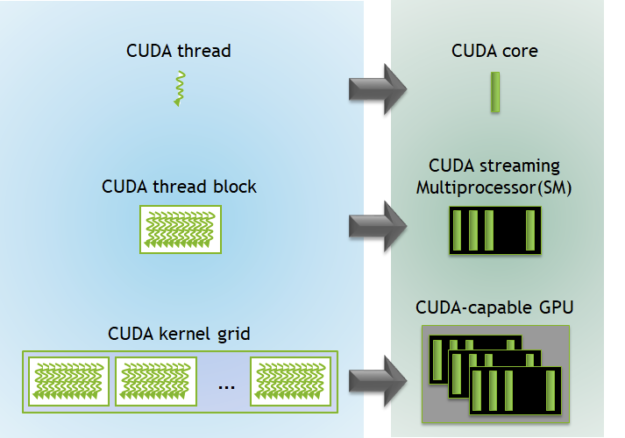
\includegraphics[width=0.5\textwidth]{./image_png/review.png}
\end{center}
\begin{center}
    \lst{auto index = threadIdx.x + blockIdx.x*blockDim.x}\\
    \vspace{0.25cm}
    \centering \includegraphics[width=\textwidth]{./images/blocks.pdf}
\end{center}

\end{frame}

%%%%%%%%%%%%%%%%%%%%%%%%%%%%%%%%%%%%%%%%%%%%
\begin{frame}[fragile]{Types of Cooperation}
%%%%%%%%%%%%%%%%%%%%%%%%%%%%%%%%%%%%%%%%%%%%
\begin{itemize}
        \item \emph{Cooperation between threads in a thread block}:
        \begin{itemize}
            \item All threads in a block run on the same SM
            \item Shared resources such as L1 cache and shared memory
            \item CUDA provides mechanisms for synchronization at the block level and lower
            \item No necessary synchronization between threads in different blocks
        \end{itemize}
        \vspace{0.5cm}
        \item \emph{Cooperation between different blocks}:
        \begin{itemize}
            \item Cooperation must occur through global memory
            \item CUDA supports \textit{atomic operations}
        \end{itemize}
\end{itemize}

\end{frame}

%%%%%%%%%%%%%%%%%%%%%%%%%%%%%%%%%%%%%%%%%%%%%%%
\begin{frame}[fragile]{Block Level Cooperation}
%%%%%%%%%%%%%%%%%%%%%%%%%%%%%%%%%%%%%%%%%%%%%%%
Cooperating through \emph{shared memory}:
\begin{itemize}
    \item Shared memory is simply a user-managed cache
    \item Threads in a block can see the same shared memory
    \item Shared memory is not visible to threads in other blocks executing on the same SM
    \item Shared memory is a limited resource (\emph{64 KB/SM on a P100}):
    \begin{itemize}
        \item Shared memory usage per block limits how many blocks can run simultaneously on an SM
        \item One thread block can allocate 64 KB for itself\dots
        \item \dots two thread blocks can allocate 32 KB each
    \end{itemize}
\end{itemize}

\end{frame}

%%%%%%%%%%%%%%%%%%%%%%%%%%%%%%%%%%%%%
\begin{frame}[fragile]{Shared Memory}
%%%%%%%%%%%%%%%%%%%%%%%%%%%%%%%%%%%%%
    \begin{itemize}
        \item What changes with different GPU architectures:
        \begin{itemize}
            \item P100: L1 cache and shared mem. have \emph{fixed} sizes
            \item A100 \& V100: L1 cache and shared mem. are now unified and their portion is \emph{configurable}
            \item 64KB/SM on a P100 and up to 128KB/SM on an A100
        \end{itemize}
        \vspace{0.25cm}
        \item What does not change from P100 upwards:
            \begin{itemize}
                \item Shared memory is divided in 32 equal memory banks, where 32-bit words map to successive banks
                \item Each memory bank has a bandwidth of 32 bits/cycle
                \item When more than one thread writes to the same bank the write operations are serialized (\emph{bank conflicts})
            \end{itemize}
        \end{itemize}

\end{frame}

%%%%%%%%%%%%%%%%%%%%%%%%%%%%%%%%%%%%%%%%%%%%
\begin{frame}[fragile]{Moving Data To and From Shared Memory}
%%%%%%%%%%%%%%%%%%%%%%%%%%%%%%%%%%%%%%%%%%%%
    \begin{itemize}
        \item P100, V100 and A100 coalesce global memory access into 32 byte transactions:
        \begin{itemize}
            \item For example, a block with 32 threads reading 1 \lst{float} per thread requires only 4 global memory transactions (if and only if the \lst{float}s are consecutive in global memory)
            \item Each of these \lst{float}s gets placed into consecutive shared memory banks without any bank conflicts
        \end{itemize}
        \vspace{0.25cm}
        \item Things to watch out for:
            \begin{itemize}
                \item When reading strided data, part of that 32 byte memory transaction will go unused
                \item This will decrease the effective memory bandwidth
            \end{itemize}
        \end{itemize}

\end{frame}

%%%%%%%%%%%%%%%%%%%%%%%%%%%%%%%%%%%%%%%%%%%%%%%%%%%%
\begin{frame}[fragile]{Copy Kernel w/ Shared Memory}
%%%%%%%%%%%%%%%%%%%%%%%%%%%%%%%%%%%%%%%%%%%%%%%%%%%%
    \begin{itemize}
        \item Do we need shared memory for this? Nope.
        \item This kernel is launched as usual.
        \item What if \lst{DECIMATE > 1}?
        \item Have we got any memory bank conflicts?
    \end{itemize}

    \begin{code}{A naive downsampling kernel}
        \begin{lstlisting}[style=boxcudatiny]
template <int BSIZE, int DECIMATE=1>
__global__ void downsample(const float* in, float* out, int n){

  // Allocate shared memory statically
  __shared__ float buffer[BSIZE];

  auto idx = threadIdx.x + blockIdx.x * BSIZE;

  // Coalesced reads - no bank conflicts
  if (idx * DECIMATE < n)
    buffer[threadIdx.x] = in[idx * DECIMATE];

  __syncthreads();

  // Coalesced writes
  if (idx < n/DECIMATE)
    out[idx] = buffer[threadIdx.x];
}
        \end{lstlisting}
    \end{code}

\end{frame}

%%%%%%%%%%%%%%%%%%%%%%%%%%%%%%%%%%%%%%%%%%%%
\begin{frame}[fragile]{Synchronizing threads}
%%%%%%%%%%%%%%%%%%%%%%%%%%%%%%%%%%%%%%%%%%%%
    What does \lst{__syncthreads()} do?
    
    \begin{itemize}
        \item All threads in the block wait for each other to finish loading data into shared memory.
        \item Only after \lst{__syncthreads()} the memory read by other threads is guaranteed to be visible to all other threads in the block.
        \item Do we need synchronization in this example? There's no thread cooperation, so ... nope!
        \item What might happen if we place the sync inside the if statement?
        
    \end{itemize}
\end{frame}

%%%%%%%%%%%%%%%%%%%%%%%%%%%%%%%%%%%%%%%%%%%%
\begin{frame}[fragile]{1D blur kernel}
%%%%%%%%%%%%%%%%%%%%%%%%%%%%%%%%%%%%%%%%%%%%
    A simple stencil operation:

    \centering $\text{out}_i = 0.25\times(\text{in}_{i-1}+2\times\text{in}_i+\text{in}_{i+1})$
    \smallskip

    \begin{itemize}
        \item Each output value is a linear combination of neighbors in input array
        \item First we look at naive implementation
    \end{itemize}

    \begin{code}{Host implementation of blur kernel}
        \begin{lstlisting}[style=boxcudatiny]
void blur(double *in, double *out, int n){
  float buff[n];
  for(auto i=1; i<n-1; ++i)
    out[i] = 0.25*(in[i-1] + 2*in[i] + in[i+1]);
}
        \end{lstlisting}
    \end{code}

\end{frame}

%%%%%%%%%%%%%%%%%%%%%%%%%%%%%%%%%%%%%%%%%%%%
\begin{frame}[fragile]{1D blur kernel on GPU}
%%%%%%%%%%%%%%%%%%%%%%%%%%%%%%%%%%%%%%%%%%%%
    Our first CUDA implementation of the blur kernel has each thread load the three values required to form its output\\
    
    \begin{code}{First implementation of blur kernel}
        \begin{lstlisting}[style=boxcudatiny]
__global__ void
blur(const double* in, double* out, int n) {
  int i = threadIdx.x + 1; // assume one thread block

  if(i<n-1) {
    out[i] = 0.25*(in[i-1] + 2*in[i] + in[i+1]);
  }
}
        \end{lstlisting}
    \end{code}

\end{frame}

%%%%%%%%%%%%%%%%%%%%%%%%%%%%%%%%%%%%%%%%%%%%
\begin{frame}[fragile]{}
%%%%%%%%%%%%%%%%%%%%%%%%%%%%%%%%%%%%%%%%%%%%
    Each thread has to load 3 values from global (?) memory to calculate its output \\

    \begin{center}
        \includegraphics[width=0.8\textwidth]{./images/blur_point_gather.pdf}
    \end{center}

    Alternatively, each value in the input array has to be added 3 times into the output array (why is this far worse than the above approach?)\\

    \begin{center}
        \includegraphics[width=0.8\textwidth]{./images/blur_point_scatter.pdf}
    \end{center}
\end{frame}

%%%%%%%%%%%%%%%%%%%%%%%%%%%%%%%%%%%%%%%%%%%%
\begin{frame}[fragile]{}
%%%%%%%%%%%%%%%%%%%%%%%%%%%%%%%%%%%%%%%%%%%%
    To take advantage of shared memory the kernel is split into two stages:
    \begin{enumerate}
        \item Load \lst{in[i]} into shared memory \lst{buffer[i]}.
        \begin{itemize}
            \item One thread has to load \lst{in[0]} \& \lst{in[n-1]}.
        \end{itemize}
        \item Use values \lst{buffer[i-1:i+1]} to compute kernel.
    \end{enumerate}

    \begin{center}
        \includegraphics[width=0.8\textwidth]{./images/blur_point_shared.pdf}
    \end{center}
\end{frame}

%%%%%%%%%%%%%%%%%%%%%%%%%%%%%%%%%%%%%%%%%%%%
\begin{frame}[fragile]{}
%%%%%%%%%%%%%%%%%%%%%%%%%%%%%%%%%%%%%%%%%%%%
    \begin{code}{Blur kernel with shared memory - single thread block}
        \begin{lstlisting}[style=boxcudatiny]
template<int BSIZE>
__global__
void blur_shared_block(const double* in, double* out, int n) {
    __shared__ double buffer[BSIZE];

    auto i = threadIdx.x + 1;

    if(i<n-1) {
        // load shared memory
        buffer[i] = in[i];
        if(i==1) {
            buffer[0] = in[0];
            buffer[n-1] = in[n-1];
        }

        __syncthreads();

        out[i] = 0.25*(buffer[i-1] + 2.0*buffer[i] + buffer[i+1]);
    }
}
        \end{lstlisting}
    \end{code}
    \begin{itemize}
        \item Do we need synchronization in this example? Yes!
        \item Thread $i$ needs to wait for threads $i-1$ and $i+1$ to load values into \lst{buffer}.
    \end{itemize}

\end{frame}

%%%%%%%%%%%%%%%%%%%%%%%%%%%%%%%%%%%%%%%%%%%%
\begin{frame}[fragile]{Declaring shared memory}
%%%%%%%%%%%%%%%%%%%%%%%%%%%%%%%%%%%%%%%%%%%%
    There are two ways to declare shared memory allocations.

    \begin{info}{Static allocation}
        When the amount of memory is known at compile time:

        \centering \lst{__shared__ double buffer[128];}
        \begin{itemize}
            \item Here there are 128 double-precision values (1024 bytes) of memory shared by all threads.
        \end{itemize}
    \end{info}

    \begin{info}{Dynamic allocation}
        When the memory is determined at run time:

        \centering \lst{extern __shared__ double buffer[];}
        \begin{itemize}
            \item Note the \lst{extern} keyword.
            \item The size of memory to be allocated is specified when the kernel is launched.
        \end{itemize}
    \end{info}

\end{frame}

%%%%%%%%%%%%%%%%%%%%%%%%%%%%%%%%%%%%%%%%%%%%
\begin{frame}[fragile]{Launching with static shared memory}
%%%%%%%%%%%%%%%%%%%%%%%%%%%%%%%%%%%%%%%%%%%%
    \begin{itemize}
        \item Always need to allocate enough shared memory for the given block size.
        \item Our \lst{blur_shared_block} kernel needed 2 extra elements ($num\_threads$ + 2)
    \end{itemize}
    \smallskip

    \begin{code}{Launching our blur\_shared\_block kernel}
        \begin{lstlisting}[style=boxcudatiny]
// Setting the block size to 128 threads
auto n = 128;
blur_shared_block<128+2>@<<<@num_blocks, n@>>>@(x0, x1, n);
        \end{lstlisting}
    \end{code}
\end{frame}

%%%%%%%%%%%%%%%%%%%%%%%%%%%%%%%%%%%%%%%%%%%%
\begin{frame}[fragile]{Launching with dynamic shared memory}
%%%%%%%%%%%%%%%%%%%%%%%%%%%%%%%%%%%%%%%%%%%%
        An additional parameter is added to the launch syntax
        \\
        \centering \lst{blur_shared``<<<``grid_dim, block_dim, shared_size``>>>``(...);}
        \begin{itemize}
            \item \lst{shared_size} is the shared memory \emph{in bytes} to be dynamically allocated \emph{per thread block}
        \end{itemize}

    \begin{code}{Launch blur kernel with shared memory}
        \begin{lstlisting}[style=boxcudatiny]
__global__
void blur_shared(double *in, double* out, int n) {
  extern __shared__ double buffer[];

  int i = threadIdx.x + 1;
  // ...
}

// in main()
auto block_dim = n;
auto size_in_bytes = (n+2)*sizeof(double);

blur_shared@<<<@1, block_dim, size_in_bytes@>>>@(x0, x1, n);
        \end{lstlisting}
    \end{code}

\end{frame}

%%%%%%%%%%%%%%%%%%%%%%%%%%%%%%%%%%%%%%%%%%%%
\begin{frame}[fragile]{Launching with static shared memory}
%%%%%%%%%%%%%%%%%%%%%%%%%%%%%%%%%%%%%%%%%%%%
    It is possible to allocate multiple variables as shared memory.
    \begin{itemize}
        \item   If the shared memory is used separately, you can use a union to ``overlap'' the storage.
        \item   Shared memory is a limited resource.
    \end{itemize}

    \begin{columns}[T]
        \begin{column}{0.48\textwidth}
            \begin{code}{separate storage}
                \begin{lstlisting}[style=boxcudatiny]
__global__
void kernel1() {
  // 1536 bytes
  __shared__ int X[128];
  __shared__ double Y[128];

  // OK
  X[i] = (int)Y[i];
}
                 \end{lstlisting}
            \end{code}
        \end{column}

        \begin{column}{0.48\textwidth}
            \begin{code}{overlapping storage}
                \begin{lstlisting}[style=boxcudatiny]
__global__
void kernel2(int n) {
  // 1024 bytes
  __shared__ union {
    int X[128];
    double Y[128];
  } buf;

  // not OK
  buf.X[i] = (int)buf.Y[i];
}
                \end{lstlisting}
            \end{code}
        \end{column}
    \end{columns}
\end{frame}

%%%%%%%%%%%%%%%%%%%%%%%%%%%%%%%%%%%%%%%%%%%%
\begin{frame}[fragile]{Finding resource usage of kernels}
%%%%%%%%%%%%%%%%%%%%%%%%%%%%%%%%%%%%%%%%%%%%
    The nvcc flag \lstterm{--resource-usage} will print the resources used by each kernel during compilation:
    \begin{itemize}
        \item shared memory
        \item constant memory
        \item registers
    \end{itemize}

    \begin{terminal}{using the \lstterm{--resource-usage} on kernels in previous slide}
    \begin{lstlisting}[style=terminal]
> nvcc --resource-usage -arch=sm_60 shared.cu 
ptxas info  : 0 bytes gmem
ptxas info  : Compiling entry function '_Z7kernel2i' for
ptxas info  : Function properties for _Z7kernel2i
0 bytes stack frame, 0 bytes spill stores, 0 bytes spill loads
ptxas info  : Used 6 registers, 1024 bytes smem, 324 bytes cmem[0]
ptxas info  : Compiling entry function '_Z7kernel1v' for
ptxas info  : Function properties for _Z7kernel1v
0 bytes stack frame, 0 bytes spill stores, 0 bytes spill loads
ptxas info  : Used 6 registers, 1536 bytes smem, 320 bytes cmem[0]
> c++filt _Z7kernel2i
kernel2(int)
    \end{lstlisting}
    \end{terminal}
    \emph{Note}: the kernel names have been mangled

\end{frame}

%%%%%%%%%%%%%%%%%%%%%%%%%%%%%%%%%%%%%%%%%%%%
\begin{frame}[fragile]{Back to our blur kernel}
%%%%%%%%%%%%%%%%%%%%%%%%%%%%%%%%%%%%%%%%%%%%
        A version of the blur kernel for arbitrarily large $n$ is provided in \lst{blur.cu} in the example code. One relevant thing to note is:
        \begin{itemize}
            \item  the \lst{in} and \lst{out} arrays use global indexes\dots
            \item  \dots and the shared memory uses thread block local indexes
        \end{itemize}

    \begin{info}{have a go at the code!}
        \begin{itemize}
            \item What's the speedup when using shared memory?
            \item \emph{Extra}: Modify the \lst{blur_shared} kernel to allocate shared memory dynamically.
        \end{itemize}
    \end{info}

\end{frame}

%%%%%%%%%%%%%%%%%%%%%%%%%%%%%%%%%%%%%%%%%%%%
\begin{frame}[fragile]{Blur kernel results}
%%%%%%%%%%%%%%%%%%%%%%%%%%%%%%%%%%%%%%%%%%%%

    \begin{info}{and all this for ... no speedup at all?}
        \begin{itemize}
            \item This kernel operates on consecutive memory.
            \item Coalesced reads and writes.
            \item Turns out that L1 cache does a pretty good job!
            \item You might get some speedup if you try this out in a very old GPU.
            \begin{itemize}
                \item GPUs prior to P100 do not cache on L1 by default.
            \end{itemize}
        \end{itemize}
    \end{info}

\end{frame}

%%%%%%%%%%%%%%%%%%%%%%%%%%%%%%%%%%%%%%%%%%%%
\begin{frame}[fragile]{Fusing kernels}
%%%%%%%%%%%%%%%%%%%%%%%%%%%%%%%%%%%%%%%%%%%%
    \begin{itemize}
        \item Sometimes a workflow uses the output of one kernel as the input of another.
        \begin{itemize}
            \item On the CPU these can be optimized by keeping the intermediate result in cache for the second kernel.
            \item On the GPU one can fuse the two operations into the same kernel and use shared memory.
        \end{itemize}
        \item An example: two concatenated stencil operations.
    \begin{code}{Naive double-blur}
        \begin{lstlisting}[style=boxcudatiny]
// Setting the block size to 128 threads
auto n = 128;
blur_shared_block<128+2>@<<<@num_blocks, n@>>>@(x0, x1, n);
blur_shared_block<128+2>@<<<@num_blocks, n@>>>@(x0, x1, n);
        \end{lstlisting}
    \end{code}
        \item Fusing these two operations will save us a round trip to global memory.
    \end{itemize}
\end{frame}


%%%%%%%%%%%%%%%%%%%%%%%%%%%%%%%%%%%%%%%%%%%%
\begin{frame}[fragile]{}
%%%%%%%%%%%%%%%%%%%%%%%%%%%%%%%%%%%%%%%%%%%%
    \begin{code}{Double blur: CUDA with shared memory}
        \begin{lstlisting}[style=boxcudatiny]
__global__ void blur_twice(const double* in, double* out, int n) {
  extern __shared__ double buffer[];

  auto block_start = blockDim.x * blockIdx.x;
  auto block_end   = block_start + blockDim.x;
  auto lid = threadIdx.x + 2;
  auto gid = lid + block_start;

  auto blur = [] (int pos, const double* field) {
    return 0.25*(field[pos-1] + 2.0*field[pos] + field[pos+1]);
  };

  if(gid<n-2) {
    buffer[lid] = blur(gid, in);
    if(threadIdx.x==0) {
        buffer[1]            = blur(block_start+1, in);
        buffer[blockDim.x+2] = blur(block_end+2, in);
    }

    __syncthreads();

    out[gid] = blur(lid, buffer);
  }
}
        \end{lstlisting}
    \end{code}
\end{frame}

%%%%%%%%%%%%%%%%%%%%%%%%%%%%%%%%%%%%%%%%%%%%
\begin{frame}[fragile]{Dissecting the speedup}
%%%%%%%%%%%%%%%%%%%%%%%%%%%%%%%%%%%%%%%%%%%%
    \begin{itemize}
        \item These types of kernels do very little math per loaded \lst{double} from global memory
        \item Total runtime heavily dominated by the global memory bandwidth
        \begin{itemize}
            \item Global memory BW: ~500GB/s (P100), ~1320GB/s (A100)
            \item Shared memory BW: ~8850GB/s (P100), ~18140GB/s (A100)
        \end{itemize}
    \end{itemize}
    \begin{columns}[T]
        \centering
        \begin{column}{0.60\textwidth}
            \centering
            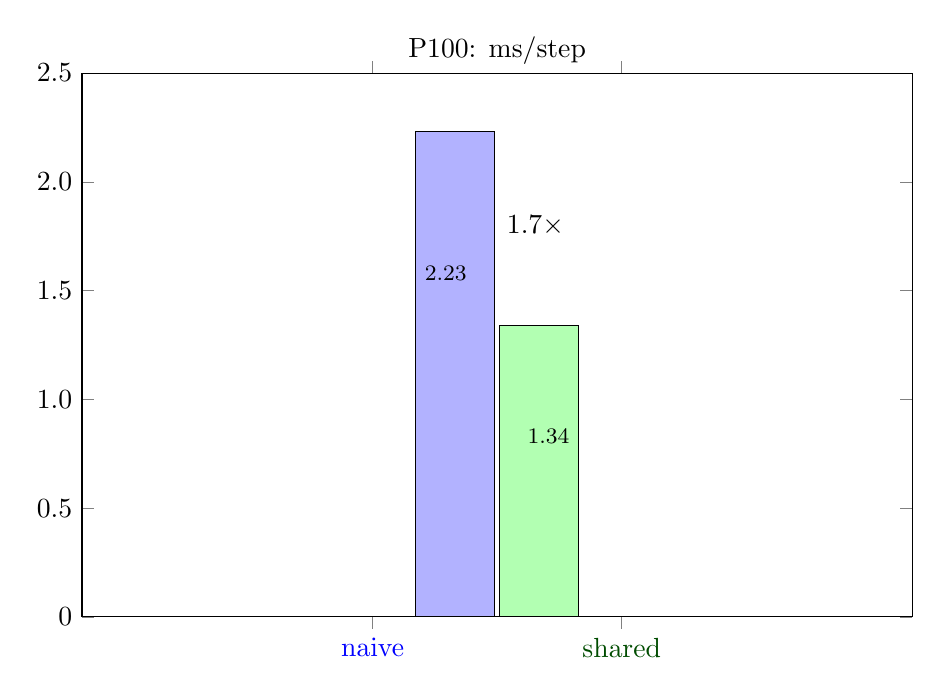
\begin{tikzpicture}
                \begin{axis}[
                    ybar,
                    height=0.7\textwidth,
                    width=\textwidth,
                    ymin=0,ymax=2.5,
                    %ticks=none,
                    ytick={0,0.5,1,1.5,2,2.5},
                    yticklabels={0,0.5,1.0,1.5,2.0,2.5},
                    title={P100: ms/step},
                    title style={yshift=-1.5ex},
                    xtick={0.94, 1.06},
                    xticklabels={\color{blue}{naive}, \color{green!30!black}{shared}}
                ]

                \addplot
                   [draw=black, fill=blue!30, bar width=1cm]
                    coordinates {(1,2.23)};
                \addplot
                   [draw=black, fill=green!30, bar width=1cm]
                    coordinates {(1,1.34)};
                \node[right] at (axis cs:1,1.8) {1.7$\times$};
                \node[above left] at (axis cs:0.99,1.5) {\footnotesize2.23};
                \node[above right] at (axis cs:1.01,0.75) {\footnotesize1.34};
                \end{axis}
            \end{tikzpicture}
        \end{column}
    \end{columns}
\end{frame}


%%%%%%%%%%%%%%%%%%%%%%%%%%%%%%%%%%%%%%%%%%%%
\begin{frame}[fragile]{Exercise: Shared Memory}
%%%%%%%%%%%%%%%%%%%%%%%%%%%%%%%%%%%%%%%%%%%%
    \begin{itemize}
        \item Finish the \lstterm{shared/string_reverse.cu} example. Assume $n\leq1024$.
        \begin{itemize}
            \item With or without shared memory.
            \item \emph{Extra}: without any synchronization.
        \end{itemize}
        \item Implement a dot product in CUDA in \lstterm{shared/dot.cu}.
        \begin{itemize}
            \item The host version has been implemented as \lst{dot_host()}
            \item Assume $n\leq1024$.
            \item \emph{Extra}: how would you extend it to work for arbitrary $n>1024$ and $n$ threads?
        \end{itemize}
    \end{itemize}

    \centering \includegraphics[width=0.5\textwidth]{./images/reduction.pdf}

\end{frame}

%%%%%%%%%%%%%%%%%%%%%%%%%%%%%%%%%%%%%%%%%%%%
\begin{frame}[fragile]{Back to Cooperation}
%%%%%%%%%%%%%%%%%%%%%%%%%%%%%%%%%%%%%%%%%%%%
    Cooperation in a GPU code can occur at multiple levels:
    \begin{itemize}
        \item Intra-block cooperation:
        \begin{itemize}
            \item Between threads in a warp;
            \item Between threads in thread block;
        \end{itemize}
        \item Inter-block cooperation:
        \begin{itemize}
            \item Between threads in grid;
            \item Between threads in different kernels.\\
        \end{itemize}
    \end{itemize}
    \bigskip
    Synchronization might be required if more than one thread wants to modify (write) one of these shared resources.
\end{frame}

%%%%%%%%%%%%%%%%%%%%%%%%%%%%%%%%%%%%%%%%%%%%
\begin{frame}[fragile]{Race conditions}
%%%%%%%%%%%%%%%%%%%%%%%%%%%%%%%%%%%%%%%%%%%%
        A race condition can occur when more than one thread attempts to access the same memory location concurrently and at least one access is a write.

\begin{columns}[T]
    \begin{column}{0.45\textwidth}
    \begin{code}{}
        \begin{lstlisting}[style=boxcudatiny]
__global__
void race(int* x) {
  ++x[0]
}

int main(void) {
  int* x =
    malloc_managed<int>(1);
  race@<<<@1, 2@>>>@(x);
  cudaDeviceSynchronize();
  // what value is in x[0]?
}
        \end{lstlisting}
    \end{code}
    \end{column}
    \begin{column}[T]{0.55\textwidth}
        \begin{center}\scriptsize
            \vspace{-0.7cm}
            \textsc{No Race} \hspace{1.5cm} \textsc{Race} \\
            \vspace{0.1cm}
        \begin{tabular}[]{|ccc|}
            \hline
             t0 &  t1 &  $x$ \\
            \hline
              R   &      &  0\\
              I   &      &  0\\
              W   &      &  1\\
                  & R    &  1\\
                  & I    &  1\\
                  & W    &  2\\
            \hline
        \end{tabular}
        \hspace{0.5cm}
        \begin{tabular}[]{|ccc|}
            \hline
             t0 &  t1 &  $x$ \\
            \hline
              R   &      &  0\\
                  &  R   &  0\\
              I   &      &  0\\
              W   &      &  1\\
                  &  I   &  1\\
                  &  W   &  1\\
            \hline
        \end{tabular}
        \end{center}
        \begin{center}
            \scriptsize
            Example where two threads \lstterm{t0} and \lstterm{t1} both increment $x$ in memory. The threads use: read (R); write (W); and increment (I).
        \end{center}
    \end{column}
\end{columns}

    \begin{itemize}
        \item Race conditions produce strange and unpredictable results.
        \item Synchronization is required to avoid race conditions.
    \end{itemize}
\end{frame}


%%%%%%%%%%%%%%%%%%%%%%%%%%%%%%%%%%%%%%%%%%%%
\begin{frame}[fragile]{Synchronization within a block}
%%%%%%%%%%%%%%%%%%%%%%%%%%%%%%%%%%%%%%%%%%%%
    Threads in the same thread block can use \lst{__syncthreads()} to synchronize on access to shared memory and global memory

    \begin{code}{synchronization on global memory}
        \begin{lstlisting}[style=boxcudatiny]
__global__
void update(int* x, int* y) {
  int i = threadIdx.x;
  if (i == 0) x[0] = 1;
  __syncthreads();
  if (i == 1) y[0] = x[0];
}

int main(void) {
  int* x = malloc_managed<int>(1);
  int* y = malloc_managed<int>(1);
  update@<<<@1,2@>>>@(x, y);
  cudaDeviceSynchronize();
  // both x[0] and y[0] equal 1
}
        \end{lstlisting}
    \end{code}

    \emph{Note}: All threads in a block must reach the \lst{__syncthreads()}
    \begin{itemize}
        \item otherwise strange things (may) happen!
    \end{itemize}
\end{frame}

%%%%%%%%%%%%%%%%%%%%%%%%%%%%%%%%%%%%%%%%%%%%
\begin{frame}[fragile]{Atomic Operations}
%%%%%%%%%%%%%%%%%%%%%%%%%%%%%%%%%%%%%%%%%%%%
    What is the output of the following code?
    \begin{code}{}
        \begin{lstlisting}[style=boxcudatiny]
#include <cstdio>
#include <cstlib>
#include <cuda.h>
#include "util.hpp"

__global__ void count_zeros(int* x, int* count) {
  int i = threadIdx.x;
  if (x[i]==0) *count+=1;
}

int main(void) {
  int* x = malloc_managed<int>(1024);
  int* count = malloc_managed<int>(1);
  count = 0;
  for (int i=0; i<1024; ++i) x[i]=i%128;

  count_zeros@<<<@1, 1024@>>>@(x, count);
  cudaDeviceSynchronize();
  printf("result %d\n", *x); // expect 8

  cudaFree(x);
  return 0;
}
        \end{lstlisting}
    \end{code}

\end{frame}

%%%%%%%%%%%%%%%%%%%%%%%%%%%%%%%%%%%%%%%%%%%%
\begin{frame}[fragile]{Atomic Operations}
%%%%%%%%%%%%%%%%%%%%%%%%%%%%%%%%%%%%%%%%%%%%
    An \emph{atomic memory operation} is an uninterruptable read-modify-write memory operation:
    \begin{itemize}
        \item Serializes contentious updates from multiple threads;
        \item \emph{The order} in which concurrent atomic updates are performed \emph{is not defined};
        \item However none of the atomic updates will be lost.
    \end{itemize}
    \vspace{-0.3cm}
    \begin{columns}[T]
        \begin{column}{0.48\textwidth}
            \begin{code}{race}
                \begin{lstlisting}[style=boxcudatiny]
__global__ void inc(int* x) {
  *x += 1;
}
                 \end{lstlisting}
            \end{code}
        \end{column}

        \begin{column}{0.48\textwidth}
            \begin{code}{no race}
                \begin{lstlisting}[style=boxcudatiny]
__global__ void inc(int* x) {
  atomicAdd(x, 1);
}
                \end{lstlisting}
            \end{code}
        \end{column}
    \end{columns}

    \begin{code}{}
        \begin{lstlisting}[style=boxcudatiny]
// pseudo-code implementation of atomicAdd
__device__ int atomicAdd(int *p, int v) {
  int old;
  exclusive_single_thread {
    old = *p; // Load from memory
    *p = old + v; // Store after adding v
  }
  return old; // return original value before modification
}
        \end{lstlisting}
    \end{code}

\end{frame}

%%%%%%%%%%%%%%%%%%%%%%%%%%%%%%%%%%%%%%%%%%%%
\begin{frame}[fragile]{Atomic Functions}
%%%%%%%%%%%%%%%%%%%%%%%%%%%%%%%%%%%%%%%%%%%%
    CUDA has a range of atomic functions, including:
    \begin{itemize}
        \item \emph{Arithmetic}:
            \lstterm{atomicAdd()}, \lstterm{atomicSub()}, \lstterm{atomicMax()}, \lstterm{atomicMin()}, \lstterm{atomicCAS()}, \lstterm{atomicExch()}.
        \item \emph{Logical}: 
            \lstterm{atomicAnd()}, \lstterm{atomicOr()}, \lstterm{atomicXor()}.
    \end{itemize}
    These functions take both 32 and 64 bit arguments
    \begin{itemize}
        \item \lstterm{atomicAdd()} gained supported for \lstterm{double} in CUDA 8 with Pascal.
        \item see the \href{https://docs.nvidia.com/cuda/cuda-c-programming-guide/index.html#atomic-functions}{\textcolor{blue}{CUDA Programming Guide}} for specific details.
    \end{itemize}
\end{frame}

%%%%%%%%%%%%%%%%%%%%%%%%%%%%%%%%%%%%%%%%%%%%
\begin{frame}[fragile]{Things to consider}
%%%%%%%%%%%%%%%%%%%%%%%%%%%%%%%%%%%%%%%%%%%%
    \begin{itemize}
        \item Atomics are slower than normal accesses:
        \begin{itemize}
            \item Performance can degrade when many threads attempt atomic operations on few memory locations.
        \end{itemize}
        \medskip
        \item Try to avoid or minimize the number of atomic operations:
        \begin{itemize}
            \item Attempt to use shared memory and structure algorithms to avoid synchronization wherever possible.
            \item Try performing operation at warp level or block level.
            \item Use atomics for infrequent, sparse and/or unpredictable global communication.
        \end{itemize}
        \medskip
        \item Further reading:
        \begin{itemize}
            \item CUDA weakly-ordered memory model
            \item Memory fence functions
        \end{itemize}
    \end{itemize}
\end{frame}

%%%%%%%%%%%%%%%%%%%%%%%%%%%%%%%%%%%%%%%%%%%%
\begin{frame}[fragile]{Exercises: Atomics}
%%%%%%%%%%%%%%%%%%%%%%%%%%%%%%%%%%%%%%%%%%%%
    \begin{itemize}
        \item What is \lstterm{shared/hist.cu} supposed to do?
        \begin{itemize}
            \item What is the output?
            \item Fix it to get the expected output.
        \end{itemize}
    \item Improve \lstterm{shared/dot.cu} to work for arbitrary $n$
    \end{itemize}
\end{frame}

\end{document}
